\documentclass[10pt]{article}
\usepackage[english]{babel}
\usepackage[utf8]{inputenc}
\usepackage[OT1]{fontenc}
\usepackage{amsfonts, amsmath, amsthm, amssymb}
\usepackage{graphicx}
\usepackage{listings}
\usepackage{hyperref}
\hypersetup{
    colorlinks=true,
    linkcolor=blue,
    filecolor=magenta,      
    urlcolor=magenta,
    pdftitle={Overleaf Example},
    pdfpagemode=FullScreen,
    }

\usepackage[margin=1in]{geometry}
\usepackage{xcolor}
\newcounter{countCode}
\lstnewenvironment{code} [1][caption=Ponme caption, label=default]{%
	\renewcommand*{\lstlistingname}{Listado} 
	\setcounter{lstlisting}{\value{countCode}} 
	\lstset{ %
	language=java,
	basicstyle=\ttfamily\footnotesize,       % the size of the fonts that are used for the code
	numbers=left,                   % where to put the line-numbers
	numberstyle=\sc,      % the size of the fonts that are used for the line-numbers
	stepnumber=1,                   % the step between two line-numbers. 
	numbersep=5pt,                 % how far the line-numbers are from the code
	numberstyle=\color{red!50!blue},
    	backgroundcolor=\color{lightgray!20},
	rulecolor=\color{blue},
	keywordstyle=\color{red}\bfseries,
	showspaces=false,               % show spaces adding particular underscores
	showstringspaces=false,         % underline spaces within strings
	showtabs=false,                 % show tabs within strings adding particular underscores
	frame=single,                   % adds a frame around the code
	framexleftmargin=0mm,
	numberblanklines=false,
	xleftmargin=5pt,
	breaklines=true,
	breakatwhitespace=true,
	breakautoindent=true,
	captionpos=t,
	texcl=true,
	tabsize=2,                      % sets default tabsize to 3 spaces
	extendedchars=true,
	inputencoding=utf8, 
	escapechar=\%,
	morekeywords={print, println, size, background, strokeWeight, fill, line, rect, ellipse, triangle, arc, save, PI, HALF_PI, QUARTER_PI, TAU, TWO_PI, width, height,},
	emph=[1]{print,println,}, emphstyle=[1]{\color{blue}}, % Mis palabras clave.
	emph=[2]{width,height,}, emphstyle=[2]{\bf\color{violet}}, % Mis palabras clave.
	emph=[3]{PI, HALF_PI, QUARTER_PI, TAU, TWO_PI}, emphstyle=[3]\color{orange!50!violet}, % Mis palabras clave.
	emph=[4]{line, rect, ellipse, triangle, arc,}, emphstyle=[4]\color{green!70!black}, % Mis palabras clave.
	%emph=[5]{size, background, strokeWeight, fill,}, emphstyle=[5]{\tt \color{red!30!blue}}, % Mis palabras clave.
	%emph={[2]sqrt,baset}, emphstyle={[2]\color{blue}}, % f(sqrt(2)), sqrt a nivel 2 se pondrá azul
	#1}}{\addtocounter{countCode}{1}}

% Pakker for kodeblokker
\usepackage{listings}
\usepackage{inconsolata} % Include the Inconsolata package
\usepackage{tabularx}
\usepackage{longtable}
\usepackage{xcolor}
\definecolor{codegreen}{rgb}{0,0.6,0}
\definecolor{codegray}{rgb}{0.5,0.5,0.5}
\definecolor{codepurple}{rgb}{0.68,0,0.12}
\definecolor{backcolour}{rgb}{0.96,0.96,0.96}

\addto\captionsnorsk{\renewcommand{\lstlistlistingname}{Koder}}
\addto\captionsnorsk{\renewcommand{\lstlistingname}{Kode}}
\lstdefinestyle{mystyle}{
    backgroundcolor=\color{backcolour},
    commentstyle=\color{codegray},
    keywordstyle=\color{codepurple},
    numberstyle=\tiny\color{codegray},
    stringstyle=\color{codegreen},
    basicstyle=\ttfamily\footnotesize\fontfamily{zi4}\selectfont, % Set Inconsolata as the font
    breakatwhitespace=false,
    breaklines=true,
    captionpos=b,
    keepspaces=true,
    numbers=left,
    numbersep=5pt,
    showspaces=false,
    showstringspaces=false,
    showtabs=false,
    tabsize=2
}

\lstset{style=mystyle}

\title{LLM Zoomcamp}
\author{Bilal Naseem\footnote{\href{https://www.linkedin.com/in/bilalnaseem96/}{https://www.linkedin.com/in/bilalnaseem96/}}}
\date{\today}
\begin{document}
\maketitle \tableofcontents 


\begin{abstract}

\end{abstract}
The following notes were made based on the course \href{https://github.com/DataTalksClub/llm-zoomcamp/tree/main}{\textbf{LLM Zoomcamp}}.
This course does not cover the theory behind LLMs and treats them as black boxes.
\section{Week 1}

\subsection{Introduction to LLM and RAG}
\footnote{\href{https://www.youtube.com/watch?v=Q75JgLEXMsM&list=PL3MmuxUbc_hIB4fSqLy_0AfTjVLpgjV3R&index=1}{Lecture 1}}A language model is a model which predicts the next word based on the words which you have typed so far. A \textbf{Large Language model} also does the same thing,
but has a lot more parameters (billions).
The input to the LLMS (text/image/video etc.) is called prompt.\\
\textbf{RAG} stands for Retrieval Augmented Generation. Retrieval means search, so a RAG system uses search to augment the generation (make it better) of the text.

\begin{figure}[h]
    \centering
    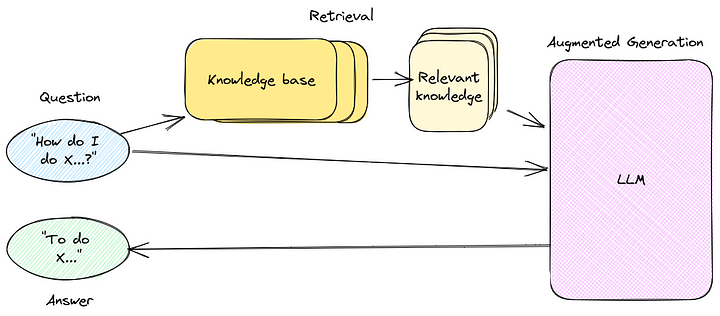
\includegraphics[width=0.6\textwidth]{media/rag_system.png}
    \caption{RAG system overview}
    \label{fig:mesh1}
\end{figure}

\subsection{Preparing the Environment}
\begin{lstlisting}
python3 -m venv myenv
source myenv/bin/activate\end{lstlisting}
\footnote{\href{https://www.youtube.com/watch?v=ozCpmkbJNJE&list=PL3MmuxUbc_hIB4fSqLy_0AfTjVLpgjV3R&index=2}{Lecture 2}}
Commands \verb|which python3| and \verb|python3 -V| can be used to check source and version of python.
\begin{lstlisting}
pip install tqdm openai elasticsearch scikit-learn pandas
pip freeze > requirements.txt\end{lstlisting}
OpenAI api key can be obtained from \href{https://platform.openai.com/api-keys}{here}.
\begin{lstlisting}
load_dotenv()
openai_key = os.getenv('OPENAI_KEY')
###
client.chat.completions.create(
    model='gpt-3.5-turbo',
    messages=[
       {
        "role": "user",
        "content": "What is up?"
       }
    ]
)\end{lstlisting}
\begin{itemize}
    \item messages is what we write to the client
\end{itemize}
\subsection{Retrieval}
xxx
\subsection{Generation with OpenAI}

\subsubsection{OpenAI API Alternatives}

\subsection{Cleaned RAG flow}

\subsection{Searching with ElasticSearch}
\end{document}

